
\section{\BookRecordIndex{T0339}稳定曲线}\label{sec:D-3}

\begin{definition}[\BookRecordIndex{T0339}稳定曲线]\label{def:D-3-1}
设 $T=(T,E,\Lambda)$ 为一棵稳定的带 $n$ 个标号的树；对每个满足
$\alpha E\beta$ 的有序对 $(\alpha,\beta)\in T\times T$，取点
$z_{\alpha\beta}\in S^2$，并取 $z_1,\ldots,z_n\in S^2$。若对每个
$\alpha\in T$，各点 $z_{\alpha\beta}$（$\alpha E\beta$）及
$z_i$（$\alpha_i=\alpha$）两两互异，则元组
\[
  \mathbf z=\bigl(\{z_{\alpha\beta}\}_{\alpha E\beta},
  \{\alpha_i,z_i\}_{1\le i\le n}\bigr)
\]
称为带 $n$ 个\BookRecordIndex{T0066}标记点的\emph{亏格零\BookRecordIndex{T0339}稳定曲线}。这些点构成 $\alpha$ 球面上的\emph{\BookRecordIndex{T0320}特殊点}集
\[
  Y_\alpha:=Y_\alpha(\mathbf z):=
  \{z_{\alpha\beta}\mid\beta\in T,\ \alpha E\beta\}
  \cup\{z_i\mid 1\le i\le n,\ \alpha_i=\alpha\}.
\]
\end{definition}

这里，稳定性条件隐含在\BookRecordIndex{T0084}带标号树稳定这一假设之中：每个 $Y_\alpha$ 至少
包含三点。因此，\BookRecordIndex{T0339}稳定曲线的自同构只有恒等映射（见下文定义~\ref{def:D-3-4}）。

\begin{remark}\label{rem:D-3-2}
引入如下记号很有用：对 $\alpha\in T$ 和 $i\in\{1,\ldots,n\}$，令
\begin{equation}\label{eq:D-3-1}
  z_{\alpha i}:=\begin{cases}
    z_i,&\alpha_i=\alpha,\\
    z_{\alpha\beta},&\alpha_i\in T_{\alpha\beta}.
  \end{cases}
\end{equation}
若 $\alpha\ne\alpha_i$，可把 $z_{\alpha i}$ 看作 $\alpha$ 球面上的唯一
\BookRecordIndex{T0191}节点，沿此\BookRecordIndex{T0191}节点可连到 $z_i$ 所在的 $\alpha_i$ 球面（见图~\ref{fig:D-3-4}）。
\end{remark}

\begin{remark}\label{rem:D-3-3}
给定互异的指标 $i,j,k\in\{1,\ldots,n\}$，式~\eqref{eq:D-2-2}
定义的顶点 $\alpha(i,j,k)$ 也可刻画为使
$z_{\alpha i},z_{\alpha j},z_{\alpha k}$ 两两互异的唯一顶点
$\alpha\in T$。这是因为当 $i\ne j$ 时，
\[
  \alpha\in[\alpha_i,\alpha_j]
  \quad\Longleftrightarrow\quad z_{\alpha i}\ne z_{\alpha j}.
\]
\end{remark}

\begin{figure}[htbp]
  \centering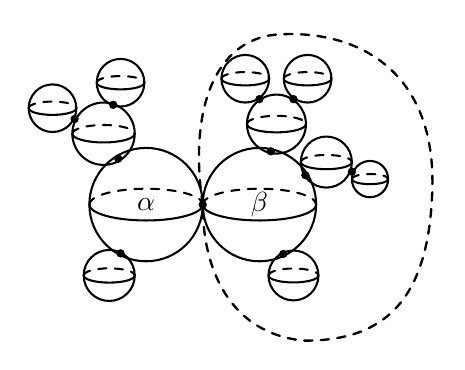
\begin{tikzpicture}[scale=.72,line width=.75pt,line cap=round]
  \newcommand{\Dsphere}[3]{%
    \pgfmathsetmacro{\Dsleft}{#1-#3}%
    \pgfmathsetmacro{\Dsy}{.28*#3}%
    \draw (#1,#2) circle (#3);
    \draw[dashed] (\Dsleft,#2) arc[start angle=180,end angle=0,x radius=#3,y radius=\Dsy];
    \draw (\Dsleft,#2) arc[start angle=180,end angle=360,x radius=#3,y radius=\Dsy];}
  \Dsphere{-2.5}{0}{1.0}
  \Dsphere{-.5}{0}{1.0}
  \Dsphere{-3.25}{1.25}{.55}
  \Dsphere{-4.15}{1.7}{.42}
  \Dsphere{-2.95}{2.15}{.42}
  \Dsphere{-3.15}{-1.25}{.45}
  \Dsphere{-.2}{1.42}{.52}
  \Dsphere{-.75}{2.22}{.42}
  \Dsphere{.35}{2.22}{.42}
  \Dsphere{.68}{.75}{.45}
  \Dsphere{1.45}{.45}{.32}
  \Dsphere{.1}{-1.25}{.44}
  \draw[dashed,line width=.85pt] (-1.5,0)
    .. controls (-1.75,1.65) and (-1.3,2.9) .. (-.2,3.0)
    .. controls (1.3,3.1) and (2.6,2.3) .. (2.55,.3)
    .. controls (2.5,-1.7) and (1.7,-2.4) .. (.3,-2.4)
    .. controls (-.9,-2.3) and (-1.5,-1.3) .. (-1.5,0);
  \foreach \p in {(-1.5,0),(-2.99,.81),(-3.76,1.51),(-3.08,1.76),
    (-2.95,-.86),(-.30,.94),(-.50,1.86),(.10,1.86),
    (.31,.52),(1.13,.58),(-.08,-.87)}
    \fill \p circle (2.1pt);
  \node at (-2.5,0) {$\alpha$};
  \node at (-.5,0) {$\beta$};
\end{tikzpicture}

  \caption{\BookRecordIndex{T0339}稳定曲线。}\label{fig:D-3-3}
\end{figure}

\begin{figure}[htbp]
  \centering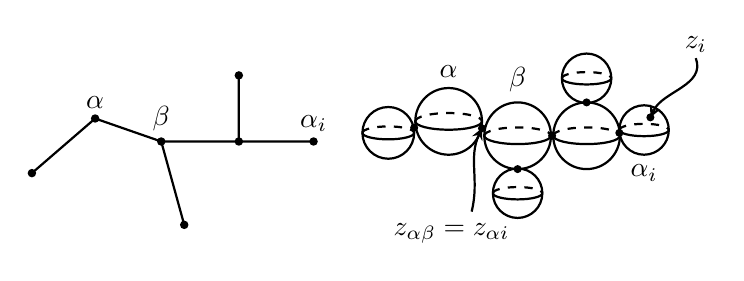
\begin{tikzpicture}[scale=.73,line width=.8pt,>=stealth]
  \coordinate (a) at (-5.3,.4); \coordinate (b) at (-4.15,0);
  \coordinate (c) at (-2.8,0); \coordinate (d) at (-1.5,0);
  \draw (-6.4,-.55)--(a)--(b)--(c)--(d);
  \draw (b)--(-3.75,-1.45) (c)--(-2.8,1.15);
  \foreach \p in {(-6.4,-.55),(a),(b),(c),(d),(-3.75,-1.45),(-2.8,1.15)}
    \fill \p circle (2.1pt);
  \node[above] at (a) {$\alpha$}; \node[above] at (b) {$\beta$};
  \node[above] at (d) {$\alpha_i$};
  \begin{scope}[shift={(2.6,0)}]
    \newcommand{\Dsmall}[3]{%
      \pgfmathsetmacro{\Dsmleft}{#1-#3}%
      \pgfmathsetmacro{\Dsmy}{.25*#3}%
      \draw (#1,#2) circle (#3);
      \draw[dashed] (\Dsmleft,#2) arc[start angle=180,end angle=0,x radius=#3,y radius=\Dsmy];
      \draw (\Dsmleft,#2) arc[start angle=180,end angle=360,x radius=#3,y radius=\Dsmy];}
    \Dsmall{-2.8}{.15}{.45}\Dsmall{-1.75}{.35}{.58}
    \Dsmall{-.55}{.1}{.58}\Dsmall{.65}{.1}{.58}
    \Dsmall{1.65}{.2}{.43}
    \Dsmall{.65}{1.1}{.43}\Dsmall{-.55}{-.9}{.43}
    \foreach \p in {(-2.35,.24),(-1.17,.23),(.05,.1),(1.22,.15),(.65,.68),(-.55,-.48)}
      \fill \p circle (2pt);
    \fill (1.76,.42) circle (2pt);
    \node[above] at (-1.75,.93) {$\alpha$};
    \node[above] at (-.55,.68) {$\beta$};
    \node[below] at (1.65,-.23) {$\alpha_i$};
    \draw[->] (-1.35,-1.22) to[out=76,in=245] (-1.17,.23);
    \node[below] at (-1.7,-1.25) {$z_{\alpha\beta}=z_{\alpha i}$};
    \draw[->] (2.55,1.45) to[out=-70,in=65] (1.76,.42);
    \node at (2.55,1.68) {$z_i$};
  \end{scope}
\end{tikzpicture}

  \caption{\BookRecordIndex{T0066}标记点。}\label{fig:D-3-4}
\end{figure}

\begin{definition}[等价]\label{def:D-3-4}
带 $n$ 个\BookRecordIndex{T0066}标记点的两条亏格零\BookRecordIndex{T0339}稳定曲线
\[
  \mathbf z=\bigl(\{z_{\alpha\beta}\}_{\alpha E\beta},
  \{\alpha_i,z_i\}_{1\le i\le n}\bigr),\qquad
  \widetilde{\mathbf z}=
  \bigl(\{\widetilde z_{\alpha\beta}\}_{\alpha\widetilde E\beta},
  \{\widetilde\alpha_i,\widetilde z_i\}_{1\le i\le n}\bigr)
\]
称为\emph{等价}，如果存在\BookRecordIndex{T0304}树同构 $f:T\to\widetilde T$ 及一族 \BookRecordIndex{T0040}Möbius 变换
$\phi=\{\phi_\alpha\}_{\alpha\in T}$，使对 $i=1,\ldots,n$ 与
$\alpha E\beta$ 有
\[
  \widetilde z_{f(\alpha)f(\beta)}=\phi_\alpha(z_{\alpha\beta}),
  \qquad\widetilde\alpha_i=f(\alpha_i),\qquad
  \widetilde z_i=\phi_{\alpha_i}(z_i).
\]
\end{definition}

对每一对等价曲线 $\mathbf z\sim\widetilde{\mathbf z}$，满足定义~\ref{def:D-3-4}
的\BookRecordIndex{T0304}树同构 $f:T\to\widetilde T$ 及 \BookRecordIndex{T0040}Möbius 变换族
$\phi=\{\phi_\alpha\}_{\alpha\in T}$ 均唯一。$f$ 的唯一性来自
$f(\alpha(i,j,k;\mathbf z))=\alpha(i,j,k;\widetilde{\mathbf z})$
对所有 $i,j,k$ 成立（见注~\ref{rem:D-3-3} 和习题~\ref{ex:D-2-5}）。
$\phi_\alpha$ 的唯一性则来自
$\phi_\alpha(z_{\alpha i})=\widetilde z_{f(\alpha)i}$，其中
$\widetilde z_{\widetilde\alpha i}$ 由式~\eqref{eq:D-3-1} 将
$T,\alpha,z_i$ 换为 $\widetilde T,\widetilde\alpha,\widetilde z_i$ 得到。

\noindent\textbf{\BookRecordIndex{T0246}模空间。}
以 $SC_{0,n}$ 表示所有带 $n$ 个\BookRecordIndex{T0066}标记点的亏格零\BookRecordIndex{T0339}稳定曲线构成的范畴。
Grothendieck--Knudsen \BookRecordIndex{T0246}模空间定义为等价关系~\ref{def:D-3-4} 下的商
\[
  \overline{\mathcal M}_{0,n}:=SC_{0,n}/\sim.
\]
其元素记为 $\zeta=[\mathbf z]$，其中 $\mathbf z$ 如定义~\ref{def:D-3-1}。
$\overline{\mathcal M}_{0,n}$ 有时也称 Deligne--Mumford 空间，不过这个名称
或许更应专用于较高亏格的情形。

可把一条亏格零\BookRecordIndex{T0339}稳定曲线 $\mathbf z$ 看成有限个二球面
$\{S_\alpha\}_{\alpha\in T}$，在 $z_{\alpha\beta}\in S_\alpha$ 处黏合，
并配以\BookRecordIndex{T0066}标记点 $z_i\in S_{\alpha_i}$。更正式地，与定义~\ref{def:D-3-1}
中的每条 $\mathbf z$ 相联系的是一张\emph{\BookRecordIndex{T0087}带节点的黎曼曲面}
\begin{equation}\label{eq:D-3-2}
  \Sigma(\mathbf z):=T\times S^2/\sim,
\end{equation}
其中 $(\alpha,z)\sim(\beta,w)$ 当且仅当或者 $\alpha=\beta$ 且 $z=w$，
或者 $\alpha E\beta$、$z=z_{\alpha\beta}$ 且 $w=z_{\beta\alpha}$。
用 $[\alpha,z]$ 表示 $(\alpha,z)\in T\times S^2$ 的等价类。
$[\alpha,z_{\alpha\beta}]=[\beta,z_{\beta\alpha}]$ 称为
$\Sigma(\mathbf z)$ 的\emph{\BookRecordIndex{T0191}节点}。各\emph{\BookRecordIndex{T0066}标记点}
$[\alpha_i,z_i]\in\Sigma(\mathbf z)$ 必须彼此互异且不同于\BookRecordIndex{T0191}节点。
此外，每个分支 $S_\alpha$ 至少包含三个\emph{\BookRecordIndex{T0320}特殊点}，即\BookRecordIndex{T0191}节点或\BookRecordIndex{T0066}标记点。
对于每对等价的 $\mathbf z,\widetilde{\mathbf z}\in SC_{0,n}$，
定义~\ref{def:D-3-4} 中唯一的元组 $(f,\{\phi_\alpha\}_{\alpha\in T})$
给出全纯微分同胚
\[
  \psi_{\widetilde{\mathbf z}\mathbf z}:\Sigma(\mathbf z)
  \longrightarrow\Sigma(\widetilde{\mathbf z}),\qquad
  \psi_{\widetilde{\mathbf z}\mathbf z}([\alpha,z])
  :=[f(\alpha),\phi_\alpha(z)],\quad\alpha\in T,\ z\in S^2.
\]
因此，每个等价类 $\zeta\in\overline{\mathcal M}_{0,n}$ 都对应空间
\begin{equation}\label{eq:D-3-3}
  \Sigma_\zeta:=\{(\mathbf z,x)\mid\mathbf z\in\zeta,\
  x\in\Sigma(\mathbf z)\}/\equiv,
\end{equation}
其中 $(\mathbf z_0,x_0)\equiv(\mathbf z_1,x_1)$ 当且仅当
$x_1=\psi_{\mathbf z_1\mathbf z_0}(x_0)$。由此，\BookRecordIndex{T0246}模空间
$\overline{\mathcal M}_{0,n}$ 可理解为各带 $n$ 个\BookRecordIndex{T0066}标记点的带\BookRecordIndex{T0191}节点黎曼曲面
$\Sigma_\zeta$ 的集合。D.7 节将对 $n=3,4,5$ 的
$\overline{\mathcal M}_{0,n}$ 作出明确描述。
